% Options for packages loaded elsewhere
\PassOptionsToPackage{unicode}{hyperref}
\PassOptionsToPackage{hyphens}{url}
%
\documentclass[
  12 pt,
  a4paper,
]{article}
\usepackage{amsmath,amssymb}
\usepackage{setspace}
\usepackage{iftex}
\ifPDFTeX
  \usepackage[T1]{fontenc}
  \usepackage[utf8]{inputenc}
  \usepackage{textcomp} % provide euro and other symbols
\else % if luatex or xetex
  \usepackage{unicode-math} % this also loads fontspec
  \defaultfontfeatures{Scale=MatchLowercase}
  \defaultfontfeatures[\rmfamily]{Ligatures=TeX,Scale=1}
\fi
\usepackage{lmodern}
\ifPDFTeX\else
  % xetex/luatex font selection
  \setmainfont[]{Times New Roman}
\fi
% Use upquote if available, for straight quotes in verbatim environments
\IfFileExists{upquote.sty}{\usepackage{upquote}}{}
\IfFileExists{microtype.sty}{% use microtype if available
  \usepackage[]{microtype}
  \UseMicrotypeSet[protrusion]{basicmath} % disable protrusion for tt fonts
}{}
\makeatletter
\@ifundefined{KOMAClassName}{% if non-KOMA class
  \IfFileExists{parskip.sty}{%
    \usepackage{parskip}
  }{% else
    \setlength{\parindent}{0pt}
    \setlength{\parskip}{6pt plus 2pt minus 1pt}}
}{% if KOMA class
  \KOMAoptions{parskip=half}}
\makeatother
\usepackage{xcolor}
\usepackage[margin=1in]{geometry}
\usepackage{graphicx}
\makeatletter
\def\maxwidth{\ifdim\Gin@nat@width>\linewidth\linewidth\else\Gin@nat@width\fi}
\def\maxheight{\ifdim\Gin@nat@height>\textheight\textheight\else\Gin@nat@height\fi}
\makeatother
% Scale images if necessary, so that they will not overflow the page
% margins by default, and it is still possible to overwrite the defaults
% using explicit options in \includegraphics[width, height, ...]{}
\setkeys{Gin}{width=\maxwidth,height=\maxheight,keepaspectratio}
% Set default figure placement to htbp
\makeatletter
\def\fps@figure{htbp}
\makeatother
\setlength{\emergencystretch}{3em} % prevent overfull lines
\providecommand{\tightlist}{%
  \setlength{\itemsep}{0pt}\setlength{\parskip}{0pt}}
\setcounter{secnumdepth}{-\maxdimen} % remove section numbering
\ifLuaTeX
\usepackage[bidi=basic]{babel}
\else
\usepackage[bidi=default]{babel}
\fi
\babelprovide[main,import]{spanish}
\ifPDFTeX
\else
\babelfont{rm}[]{Times New Roman}
\fi
% get rid of language-specific shorthands (see #6817):
\let\LanguageShortHands\languageshorthands
\def\languageshorthands#1{}
\ifLuaTeX
  \usepackage{selnolig}  % disable illegal ligatures
\fi
\usepackage{bookmark}
\IfFileExists{xurl.sty}{\usepackage{xurl}}{} % add URL line breaks if available
\urlstyle{same}
\hypersetup{
  pdftitle={INTRODUCCIÓ ALS SISTEMES INFORMÀTICS},
  pdfauthor={Tomàs Ferrandis Moscardó},
  pdflang={es-ES},
  hidelinks,
  pdfcreator={LaTeX via pandoc}}

\title{INTRODUCCIÓ ALS SISTEMES INFORMÀTICS}
\author{Tomàs Ferrandis Moscardó}
\date{2024-08-29}

\begin{document}
\maketitle

{
\setcounter{tocdepth}{2}
\tableofcontents
}
\setstretch{1.5}
\newpage
\renewcommand\tablename{Tabla}

\section{1. El sistema informàtic}\label{el-sistema-informuxe0tic}

Un sistema informàtic és un conjunt integrat de components, tant físics
com digitals, dissenyats per a la captura, emmagatzematge, processament
i comunicació d'informació.

Aquest sistema està compost per 3 tipus d'elements:

\begin{itemize}
\item
  Hardware (maquinari)
\item
  Software (programari)
\item
  Usuaris
\end{itemize}

\subsection{1.1 Tipus de sistemes
informàtics}\label{tipus-de-sistemes-informuxe0tics}

\begin{itemize}
\tightlist
\item
  \textbf{Sistemes personals}: Inclouen PC (ordinadors de sobretaula o
  Personal Computer), portàtils, tauletes i smartphones.
\item
  \textbf{Sistemes empresarials}: Com ara servidors, mainframes i
  sistemes de computació en núvol, que suporten les operacions d'una
  organització.
\item
  \textbf{Sistemes empotrats}: Sistemes informàtics especialitzats que
  es troben dins d'altres dispositius com electrodomèstics, cotxes i
  dispositius mèdics.
\end{itemize}

\section{2. Components hardware}\label{components-hardware}

Els components hardware constitueixen la part física dels sistemes
informàtics, incloent dispositius que són visibles, tangibles així com
la lògica de la electrònica digital.

\subsection{2.1 Elements funcionals
princIpals}\label{elements-funcionals-principals}

\begin{itemize}
\tightlist
\item
  \textbf{Processador (CPU)}: L'element principal que executa les
  instruccions dels programes.
\item
  \textbf{Memòria}: Inclou la RAM (memòria d'accés aleatori) per a
  l'emmagatzematge temporal.
\end{itemize}

\subsection{2.2 Perifèrics (Unitat E/S)}\label{perifuxe8rics-unitat-es}

Els perifèrics són dispositius connectats a l'ordinador que faciliten la
interacció amb el sistema o amplien les seves funcionalitats. Es poden
classificar en diverses categories:

\subsubsection[2.2.1 Dispositius d'entrada/eixida** pròpiament
dits]{\texorpdfstring{2.2.1 Dispositius d'entrada/eixida** pròpiament
dits\footnote{Alguns autors usen el terme \emph{Dispositius
  d'entrada/eixida} en un sentit genèric abarcant a tots els
  \emph{Perifèrics} donat que la Unitat Funcional que abarca tots els
  perifèrics és la Unitat d'E/S.}}{2.2.1 Dispositius d'entrada/eixida** pròpiament dits}}\label{dispositius-dentradaeixida-pruxf2piament-dits1}

\begin{itemize}
\tightlist
\item
  \textbf{Entrada}: Dispositius que permeten introduir dades o
  comandaments a l'ordinador.

  \begin{itemize}
  \tightlist
  \item
    \emph{Exemples}: Teclats, ratolins, escàners, micròfons.
  \end{itemize}
\item
  \textbf{Eixida}: Dispositius que mostren o emeten informació
  processada per l'ordinador.

  \begin{itemize}
  \tightlist
  \item
    \emph{Exemples}: Monitors, impressores, altaveus, projectors.
  \end{itemize}
\item
  \textbf{Entrada i eixida}. Dispositius que poden fer les dues funcions
  adés esmentades alhora:

  \begin{itemize}
  \tightlist
  \item
    \emph{Exemples}: Pantalla tàctil.
  \end{itemize}
\end{itemize}

\subsubsection{2.2.2 Dispositius de
magatzematge}\label{dispositius-de-magatzematge}

\begin{itemize}
\tightlist
\item
  Dispositius que magatzemem dades de forma permanent.

  \begin{itemize}
  \tightlist
  \item
    \emph{Exemples}: Discs durs (HDD, SSD), unitats de disc òptic
    (CD/DVD), memòries USB, targetes de memòria.
  \end{itemize}
\end{itemize}

\subsubsection{2.2.3 Dispositius de
comunicació}\label{dispositius-de-comunicaciuxf3}

\begin{itemize}
\tightlist
\item
  Dispositius que permeten la transmissió de dades entre ordinadors o
  altres dispositius.

  \begin{itemize}
  \tightlist
  \item
    \emph{Exemples}: Mòdems, targetes de xarxa, routers, adaptadors
    Wi-Fi, adaptador
  \end{itemize}
\end{itemize}

\subsection{2.2 Busos.}\label{busos.}

Un bus és una línia o conjunt que pot tenir dos estats (0/1).

\begin{itemize}
\tightlist
\item
  D'adreces. Serveixen per seleccionar quina posició de a memòria volem
  accedir
\item
  De dades. Serveiexen per llegir les dades de les posicions on hem
  accedit o per enviar les dades a escriure.
\item
  De control. Envien senyal com ara Read/Write
\end{itemize}

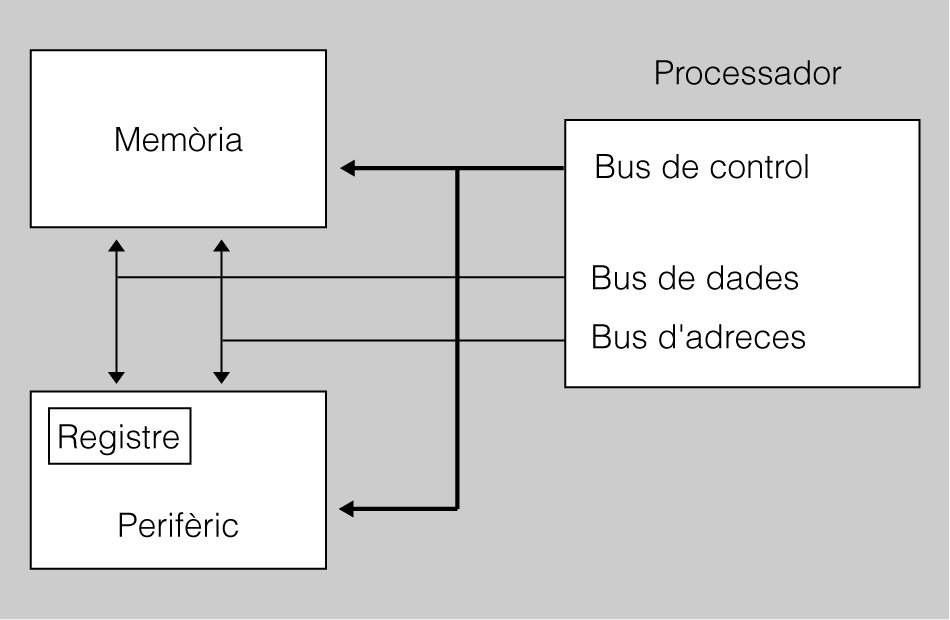
\includegraphics{recursos/esquema.png}

\subsection{2.3 Elements auxiliars}\label{elements-auxiliars}

No afecten a la capacitat del sistema però són necessaris per a que este
funcione.

\begin{itemize}
\tightlist
\item
  \textbf{Plaques base}: Suport físic per als components i
  connectivitats.
\item
  \textbf{Alimentació elèctrica}: Subministra l'energia necessària per
  al funcionament del sistema.
\item
  \textbf{Torres, racks}: Conté el PC o servidor.
\end{itemize}

\section{3. Programari d'un sistema
informàtic}\label{programari-dun-sistema-informuxe0tic}

El programari és l'equipament lògic d'un sistema informàtic, que inclou
els programes i aplicacions que permeten realitzar tasques específiques.

\subsection{3.1 Tipus de programari}\label{tipus-de-programari}

\begin{itemize}
\item
  \textbf{Programari de sistema}: Com els sistemes operatius (Windows,
  Linux), software base per a donar serveis al programari d'aplicació,
  ferramentes que podem instal·lar per a feines de gestió o
  administració del sistema o proves

  \begin{itemize}
  \tightlist
  \item
    El software que usa un tècnic o un administrador d'una xarxa
  \item
    Exemples: Tots els SO, PacketTracer, Gparted, MySQL,
    net-tools\ldots{}
  \end{itemize}
\item
  \textbf{Programari d'aplicació}: Inclou programes per a tasques
  específiques com processadors de textos, fulls de càlcul i navegadors
  web.

  \begin{itemize}
  \tightlist
  \item
    El software que usa un usuari final.
  \item
    Exemples: Paquets d'ofimàtica, ERP, jocs, navegadors\ldots{}
  \end{itemize}
\item
  \textbf{Programari de desenvolupament}: Eines per crear altres
  programes, com entorns de desenvolupament integrats (IDE).

  \begin{itemize}
  \item
    El software que usa un programador.
  \item
    Exemples: Visual Studio, RStudio, Eclipse, NetBeans, Git,
    GitHub\ldots{}

    \textbf{2.2 Elements funcionals auxiliars}

    \begin{itemize}
    \tightlist
    \item
      \textbf{Plaques base}: Suport físic per als components i
      connectivitats.
    \item
      \textbf{Alimentació elèctrica}: Fonts d'alimentació o SAI per
      subministrar l'energia necessària per al funcionament del sistema.
    \item
      \textbf{Elements de refrigeració}
    \item
      \textbf{Torres, racks.}
    \end{itemize}
  \end{itemize}
\end{itemize}

\subsection{3.2 Llicències de
programari}\label{llicuxe8ncies-de-programari}

Sense entras a fons, veiem algunes de les llicències més habituals i
alguns exemples de software que s'usa en els cicles formatius
d'informàtica.

\subsubsection{Llicències de Programari Lliure i de Codi
Obert}\label{llicuxe8ncies-de-programari-lliure-i-de-codi-obert}

Aquestes llicències permeten als usuaris utilitzar, copiar, modificar i
distribuir el programari lliurement. Alguns exemples inclouen:

\begin{itemize}
\tightlist
\item
  \textbf{GPL (GNU General Public License)}: Utilitzada per projectes
  com el SO Linux o el paquet LibreOffice

  \begin{itemize}
  \tightlist
  \item
    Existeixen varietats de la GPL com Odoo, un ERP de codi obert de
    llicencai AGPLv3.
  \end{itemize}
\item
  \textbf{MIT License}: Una llicència molt permissiva que s'utilitza en
  programes com JavaScript\textbf{, }jQuery, Bootstrap o React.
\item
  \textbf{Apache License}: Utilitzada per projectes com Apache HTTP
  Server.
\end{itemize}

\subsubsection{Llicències Comercials}\label{llicuxe8ncies-comercials}

Aquestes llicències requereixen la compra d'una llicència per a
utilitzar el programari. Exemples comuns inclouen:

\begin{itemize}
\tightlist
\item
  \emph{Exemples}: Microsoft Office, Adobe Photoshop, Oracle
  Database\ldots amb llicències comercials.
\end{itemize}

\subsubsection{Llicències Shareware}\label{llicuxe8ncies-shareware}

Aquestes llicències permeten l'ús gratuït del programari durant un
període de prova limitat o amb funcionalitats restringides. Alguns
exemples són:

\begin{itemize}
\tightlist
\item
  \emph{Exemples:} WinRAR (per a la compressió de fitxers), Sublime Text
  (Editor de text amb una versió de prova disponible).
\end{itemize}

\paragraph{\texorpdfstring{\textbf{Llicències
Freeware}}{Llicències Freeware}}\label{llicuxe8ncies-freeware}

Aquestes llicències permeten l'ús gratuït del programari sense límits de
temps, però sovint no permeten la modificació del codi font.

\begin{itemize}
\tightlist
\item
  \emph{Exemples:} Skype (Aplicació per a trucades de veu i vídeo), AVG
  Antivirus Free (Versió gratuïta d'un programa antivirus).
\end{itemize}

\subsubsection{Llicències de Programari de Prova
(Trial)}\label{llicuxe8ncies-de-programari-de-prova-trial}

Similar a les llicències shareware, però generalment ofereixen totes les
funcionalitats del programari durant un període de prova limitat.

\begin{itemize}
\tightlist
\item
  \emph{Exemples:} AutoCAD ( per a disseny assistit per ordinador),
  Adobe Premiere Pro (Programari de edició de vídeo).
\end{itemize}

\subsubsection{Llicències de Programari
Propietari}\label{llicuxe8ncies-de-programari-propietari}

Aquestes llicències són les més restrictives.

\begin{itemize}
\tightlist
\item
  \emph{Exemples:} els SO macOS, MS Windows; SAP ERP, Microsoft Dynamic
  365, Oracle ERP
\end{itemize}

Aquestes categories reflecteixen diferents models de distribució i ús
del programari, amb variacions en termes de cost, accés al codi font i
drets de modificació i redistribució.

\subsection{3.3 Creative Commons}\label{creative-commons}

Creative Commons (CC) és una organització sense ànim de lucre dedicada a
reduir les barreres legals per a compartir treballs. No és un
intermediari ni gestor de dets, sols proporciona la ferramenta per a que
cada autor puga definir quins usos permet i quins no sobre cada obra
seua.

Les llicències Creative Commons es basen en quatre condicions bàsiques
que es poden combinar:

\begin{enumerate}
\def\labelenumi{\arabic{enumi}.}
\tightlist
\item
  \textbf{Reconeixement (BY)}: Permet l'ús de l'obra sempre que
  s'atribueixi l'autoria.
\item
  \textbf{No Comercial (NC)}: Prohibeix l'ús comercial de l'obra.
\item
  \textbf{Sense Obres Derivades (ND)}: Prohibeix la creació d'obres
  derivades.
\item
  \textbf{Compartir Igual (SA)}: Les obres derivades han de ser
  licenciades sota els mateixos termes que
  l'original.
\includegraphics{recursos/cc-icons.jpg}
\end{enumerate}

Amb aquestes condicions es poden crear les següents sis llicències:

\begin{enumerate}
\def\labelenumi{\arabic{enumi}.}
\tightlist
\item
  \textbf{CC BY}: Permet l'ús comercial i la creació de derivats, sempre
  que es reconegui l'autoria.
\item
  \textbf{CC BY-NC}: Permet la creació de derivats només per ús no
  comercial.
\item
  \textbf{CC BY-NC-SA}: Permet derivats només per ús no comercial, amb
  la mateixa llicència que l'original.
\item
  \textbf{CC BY-NC-ND}: No permet derivats ni ús comercial.
\item
  \textbf{CC BY-SA}: Permet l'ús comercial i la creació de derivats, amb
  la mateixa llicència que l'original.
\item
  \textbf{CC BY-ND}: Permet l'ús comercial, però no la creació de
  derivats.
\end{enumerate}

\subsection{3.4 Normativa legal}\label{normativa-legal}

Inclou les lleis i regulacions que afecten l'ús i distribució de
programari, com la propietat intel·lectual, els drets d'autor i les
polítiques de privacitat.

\section{4 L'ELEMENT HUMÀ DEL
SISTEMA}\label{lelement-humuxe0-del-sistema}

Com ja hem dit adés, a banda del software i el hardware existeix un
tercer element en tot sistema informàtic: l'element humà. Les perosnes
podem qualificar-les, grosso modo, en 3 grups:

\begin{itemize}
\item
  Els responsables de la crear software (programadors, dissenyadors,
  analistes\ldots). Més familiaritzats am el software ded
  desenvolupament.
\item
  Els responsables de la instal·lació, configuració i manteniment del
  sistema (administradors de xarxa, tècnics de manteniment\ldots) . Més
  familiaritzats amb el software de sistema i el hardware.
\item
  Els usuaris finals del sistema. Realitzaran les tasques específiques
  que l'organització necessites amb el software d'aplicació (factures,
  informes, edició de vídeo, maquetació, càlculs estadístics, tractament
  de dades\ldots{} )
\end{itemize}

\begin{itemize}
\tightlist
\item
\end{itemize}

\end{document}
